%!TEX root = main.tex
\chapter{Natural Feature Point}\label{chapter:Natural Feature Point}
As it was mentioned in the introduction, there are two major methods for 3D tracking: feature-based and marker-based techniques. Marker-based 3D tracking system, requires the marker and prior knowledge about the environment to estimate the pose of camera. Some times due to some restriction about the environment (e.g. outdoor environment) and tracking situation, this task is hard ot do or impossible. Hence, it is better to rely on the features that naturally are extracted from images. In this approach, more meta informations such as a model of scene object, a set of planer parts and some information about the camera is necessary. To make this procedure independent of 3D scene models, Vincent lepetit and Pascal Fua \cite{lepetit2005monocular} introduced a method that can explored simultaneously both camera trajectory (tracking) and 3D world map of environment (mapping). \\
For the feature-based 3D Tracking, the whole literature in this subject can be organized into two big families regarding to the properties of the image that we want to use.
\begin{itemize}
\item Edge-Based methods investigate the areas with the highest value of gradient that represents edges. These methods try to make an accurate match between the projection of 3D edges in the real world and these gradient points. RAPID, Explicit Edge Extraction, and Direct Optimization on Gradient are some algorithms in this area. 
% http://en.wikipedia.org/wiki/Feature_detection_(computer_vision) for example.
\item The other methods investigate on the information that can be extracted directly from the pixels of image. These can be derived from optical flow, template matching, and feature points techniques.
% TODO: check the comma
\end{itemize}

\section{Feature Point Method (Corner-Based)}
% TODO: check the first params
% TODO convert all feature point to the feature point and feature point
Despite of Edge-Based methods that need an overall view of the whole image to find the high gradient points and contours, The feature point-based methods just use of localized features and it is the difference key between these two approaches. An feature point is a intersection of two edges that represents a point in which the direction of these two edges changed. Consequently, the gradients of this point have a huge amount in both directions. This property can be used to detect the feature point easily.\\
Both Edge-Based and feature Point-Based techniques rely on the matching the features among the frames independent of other points. They also can handle the partial occlusions and matching errors problems and are invariant to change of illumination. The advantage of feature point-based methods compared to edge-based methods is that they are not affected by the background clutter. In fact feature points can be uniquely recognizable between all image pixels.\\
% For the rest of this master thesis, instead of feature points, we used of feature points or feature points terms.\\
Comparing all pixels of two or more images, one by one, is very complex and requires enormous computational time. Instead of this method, the unique feature points are detected (feature detection) from images and then coded into a vector of binary or float numbers (feature extraction). this vector is called the feature descriptor.\\

\subsection{Feature Detection}
 The efficient detection of feature point is a crucial step for many computer vision applications. For detection of features points, attention to some properties of points should be considered as follows: \cite{forstner1986feature}
\begin{enumerate}
  \item The feature points are represented by a surrounding patch around the center. This patch should be textured.
  \item Two neighbor feature points, should be different.
  \item Two almost similar feature points (usually neighbor or from same pattern) should be ignored.
  \item The feature selection operation, should have the same result and performance in all images. It means if a point was selected as a feature point in one section of the image, it should also be selected as a feature point in the same section of the other images.
\end{enumerate}
For the first time, Harris and Stephen \cite{harris1988combined} published a new method for feature detection regarding to fact that the corner of feature point represents a variation in the gradient of the point in two directions. They used this variation for detect the feature point.\\
Currently, with the advances in the field of computer vision, many new techniques for feature detection have been developed for variety of image conditions. Some of the most versatile and popular feature detector are:
\begin{itemize}
\item SIFT \cite{lowe2004distinctive} based on Difference of Gaussians (DoG).
\item SURF \cite{bay2006surf} is an instance of 2D Haar wavelet.
\item FAST \cite{rosten2010faster} use of heuristic model for feature point and machine learning techniques.
% TODO: more deatil
\end{itemize}
% TODO: some methods support both feature detection and extraction but some one not

\subsection{Feature Extraction}
Once feature points are located, we are featureed in describing a patch which surrounds the feature point as the feature descriptor. The most well-known descriptor is SIFT \cite{lowe2004distinctive}: A 128-dimensional vector is obtained from a grid of histogram. It is a powerful descriptor and robust to illumination and change of view. Another approach that is wildly used at the moment is SURF \cite{bay2006surf}. Its idea based on local gradient histogram and it has similar performance as SIFT. The advantage of SURF algorithm over SIFT is that it is faster with less memory. Both of these approaches describe a feature point with a vector of float numbers. The SIFT uses with 128-dimensional vector and SURF with 64 or 128-dimensional vector.\\
In 2010, Calonder \textit{et al.} in \cite{calonder2010brief} showed that it is possible to decrease the dimensionality of a feature descriptor by directly building a shorter binary descriptor in which all bits are pairwise independent. This new algorithm is called BRIEF. Representing the feature descriptor as a binary vector has the advantage of using of Hamming distance (bitwise XOR) instead of Euclidean distance for matching of the descriptors. The negative point of BRIEF algorithm however is that the result descriptor is not invariant to scale and rotation changes. After the BRIEF, both BRISK \cite{leutenegger2011brisk} and FREAK \cite{alahi2012freak} were developed that are state-of-the-art algorithms that rely on binary descriptors and are also invariant to scale and rotation. BRISK and FREAK are inspired by intensity comparisons around a feature point and human visual system (especially retina) respectively.

\subsection {KAZE and A-KAZE}
KAZE (Japanese word meaning \emph{wind}) \cite{alcantarilla2012kaze} feature is a new 2D multi-scale feature detection and description that its algorithm rely on nonlinear scale space. Previous methods such as SIFT or SURF find features in the Gaussian scale space (particular instance of linear diffusion). However, Gaussian blurring does not respect the natural boundaries of objects and smooths in the same degree details and noise when evolving the original image through the scale space.\\
By means of nonlinear diffusion we can detect and describe features in nonlinear scale spaces keeping important image details and removing noise as long as we evolve the image in the scale space. We use variable conductance diffusion which is one of the simplest cases of nonlinear diffusion. The nonlinear scale space is build efficiently by means of Additive Operator Splitting (AOS) schemes, which are stable for any step size and are parallelizable.\\
A-KAZE (Accelerated-KAZE) \cite{alcantarilla2011fast} Features uses a novel mathematical framework called Fast Explicit Diffusion (FED) embedded in a pyramidal framework to speed-up dramatically the nonlinear scale space computation. In addition, we compute a robust Modified-Local Difference Binary (M-LDB) descriptor that exploits gradient information from the nonlinear scale space. A-KAZE obtains comparable results to KAZE in some datasets, while being several orders of magnitude faster.\\
% TODO: check the speed
Despite of moderate increase in computational time, especially compare to SURF, but the AKZE feature algorithms is a forward step in performance and accuracy for both detection and description against previous state-of-the-art algorithms such as SURF, SIFT, BRISK and FREAK.
The below graphs are taken form computer-vision-talks weblog \footnote{\url{http://computer-vision-talks.com/articles/2013-03-17-porting-kaze-features-to-opencv/}} and prepared by OpenCV Comparison Tool \footnote{\url{https://github.com/BloodAxe/OpenCV-Features-Comparison}}. It compares the KAZE feature with the other well-known algorithms from several aspects of invariance such as rotation, scale and brittleness and robustness to blur. As you can see, in all cases, the result of KAZE is strongly effective and better than others. 

\begin{figure}[H]
\begin{tabular}{cc}
  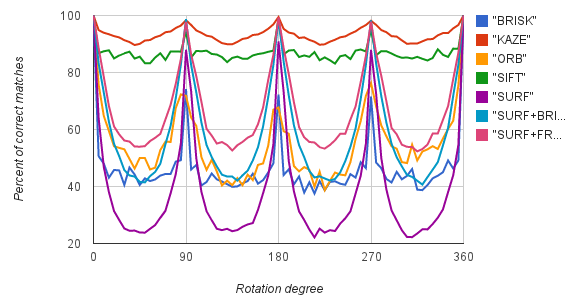
\includegraphics[width=75mm]{figures/rotation_KAZE} &  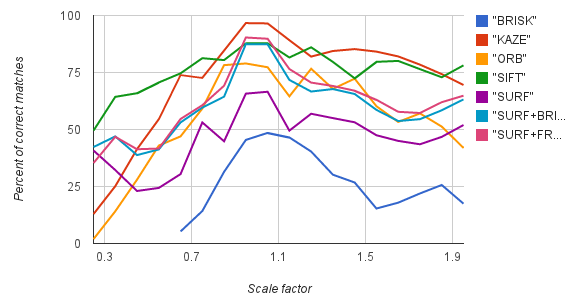
\includegraphics[width=75mm]{figures/scale_KAZE} \\
(a) Rotation Test & (b) Scale Invariance \\[6pt]
 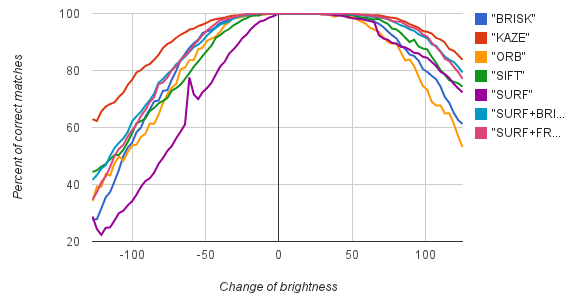
\includegraphics[width=75mm]{figures/brightness_KAZE} &  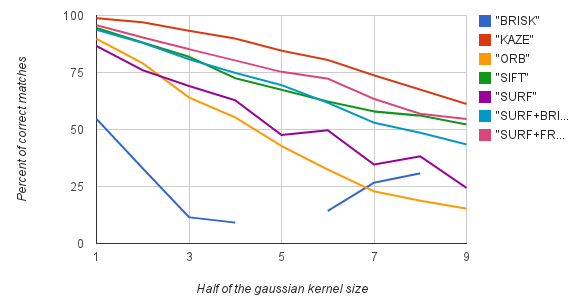
\includegraphics[width=75mm]{figures/blur_KAZE} \\
(c) Brittleness Invariance & (d) Robustness to Blur \\[6pt]
\end{tabular}
\caption{The comparison of KAZE and other well-know feature descriptions}\label{fig:compare_kaze}
\end{figure}

As we mentioned in the description of A-KAZE, it uses two new algorithms (FED and M-LDB) and consequently the computation cost for detection and description decrease dramatically. It also extends to support four different types of extracted descriptors (\detokenize{Descriptor_KAZE, Descriptor_KAZE_upright, Descriptor_MLDB and Descriptor_MLDB_upright)}) depending on image properties. In the next graph, a comparison between four top binary descriptors, A-KAZE, KAZE, BRISK, FREAK, is shown. It also was prepared by computer-vision-talks weblog. All methods are tested for a variety of environments and conditions.
% $$(Descriptor_KAZE, Descriptor_KAZE_upright, Descriptor_MLDB and Descriptor_MLDB_upright)$$

\begin{figure}[H]
\begin{tabular}{cc}
  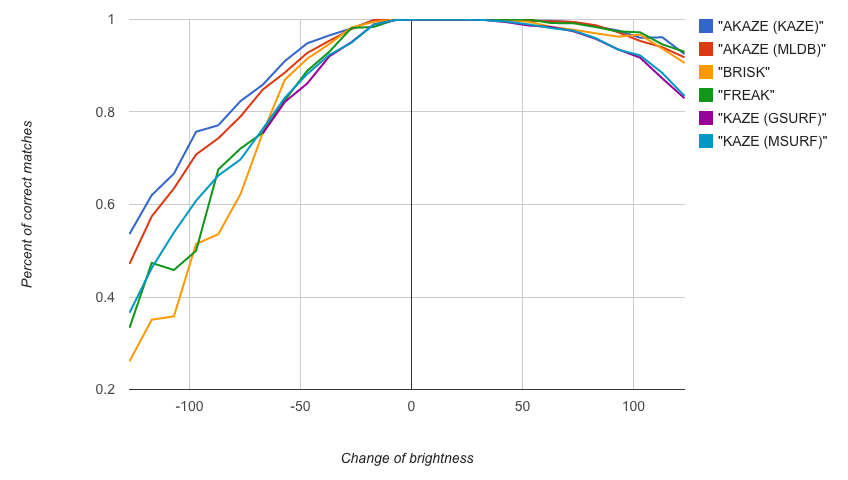
\includegraphics[width=75mm]{figures/brithness_akaze} &  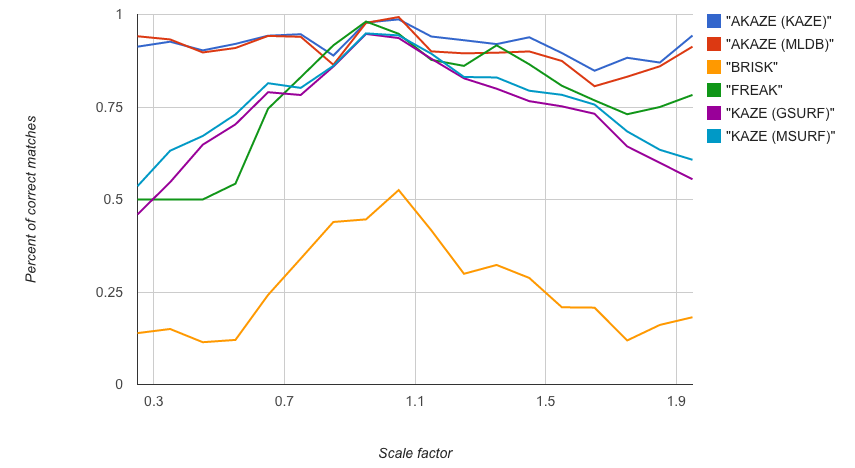
\includegraphics[width=75mm]{figures/scale_akaze} \\
(a) Brittleness Invariance & (b) Scale Invariance \\[6pt]
\multicolumn{2}{c}{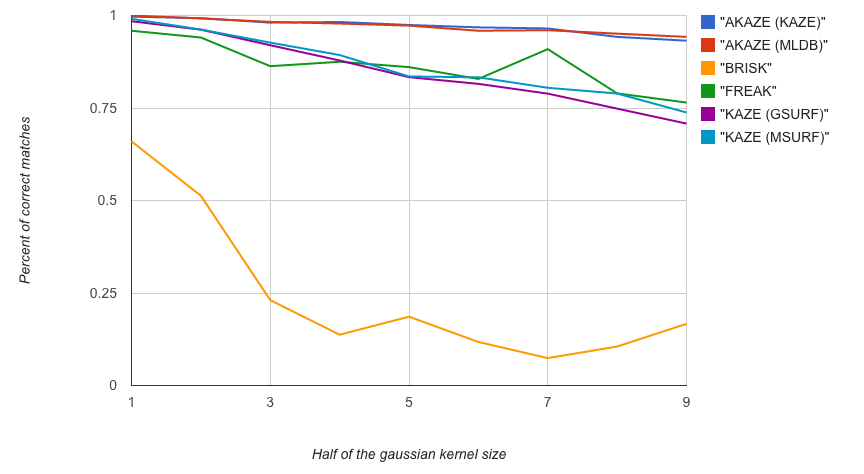
\includegraphics[width=75mm]{figures/blur_akaze} }\\
\multicolumn{2}{c}{(e) Robustness to Blur}
\end{tabular}
\caption{The comparison between KAZE and A-KAZE}\label{fig:compare_kaze_and_A-kaze}
\end{figure}

% TODO : add new test and combines with next paragraph.
Beside of the original author's implementation \footnote{\url{https://github.com/pablofdezalc/akaze}}, both KAZE and A-KAZE are ported to the new version of OpenCV 3.0 and boosted by OpenCL. In this master thesis, the OpenCV's A-KAZE is utilized for both feature detection and description procedures. The parameters of A-KAZE optimized based of our requirement and listed as below table:

\begin{table}[H]
  \caption{A-KAZE value parameters in OpenCV 3.0}
  \begin{tabular}{| c | c | c | c | c | c | c |}
      \hline
      descriptor type & descriptor size & descriptor channels & threshold & octaves & sublevels & diffusivity \\ \hline \hline
      Descriptor dump & Full & 3 & 0.001 & 4 & 4 & dump \\ \hline
  \end{tabular}
\end{table}

In this master thesis we were looking for a best feature descriptor that should be invariant to brightness, scale, rotation and be robust to blur. Between all feature detectors and extractors already mentioned here, the KAZE (Japanese word meaning \emph{wind}) and especially A-KAZE feature detector and extractor was selected. Right now it has the best result among all algorithms in this subject. The structure of its descriptor is binary and is added to the new version of OpenCV 3.0 \footnote{\url{http://docs.opencv.org/trunk/modules/features2d/doc/feature_detection_and_description.html}}.
